% Generated by plsimcount.pfseeds -- do not edit; regenerate instead.
% figure: B-all-by-formula -- Every formula at measured r; median over seeds [1, 2, 3, 4, 5], bars = min..max
% metric=cnot gatebase=cz merged
% seed 1: git_commit=8dd1b68c1faeffb1fb64439f6d7c9c5df3cf51a5 git_dirty=False
% seed 2: git_commit=8dd1b68c1faeffb1fb64439f6d7c9c5df3cf51a5 git_dirty=False
% seed 3: git_commit=8dd1b68c1faeffb1fb64439f6d7c9c5df3cf51a5 git_dirty=False
% seed 4: git_commit=8dd1b68c1faeffb1fb64439f6d7c9c5df3cf51a5 git_dirty=False
% seed 5: git_commit=8dd1b68c1faeffb1fb64439f6d7c9c5df3cf51a5 git_dirty=False
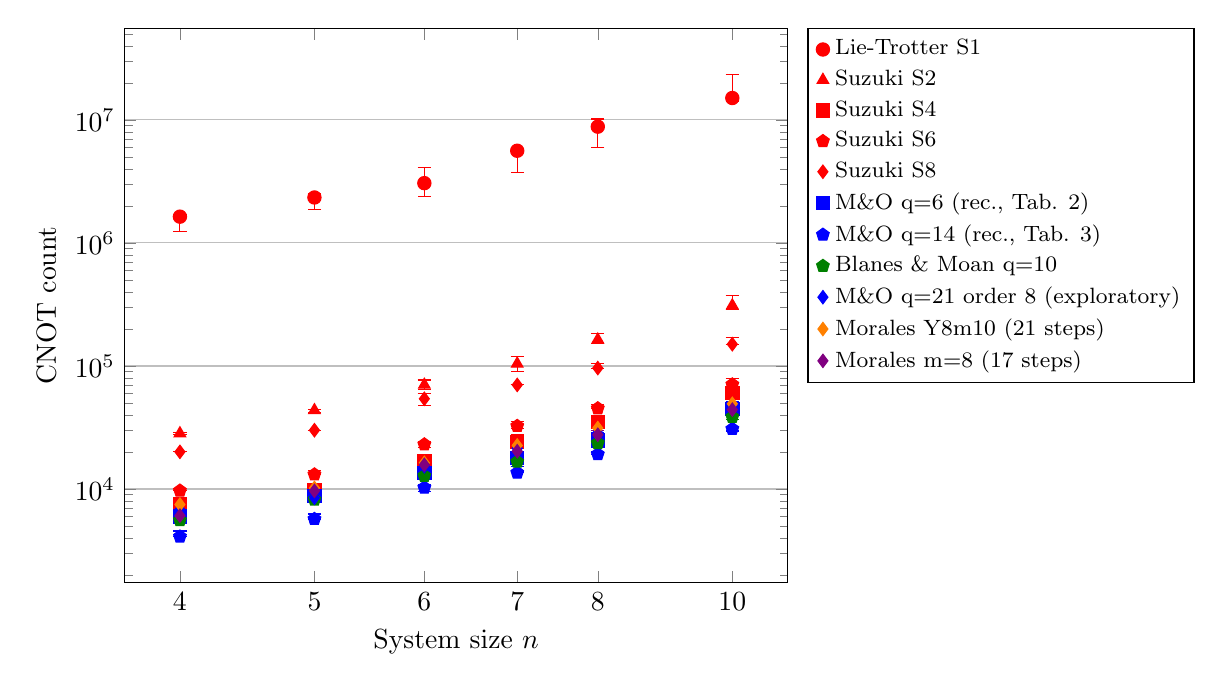
\begin{tikzpicture}
  \begin{loglogaxis}[
    width=10cm,
    xlabel={System size $n$},
    ylabel={CNOT count},
    xtick={4,5,6,7,8,10},
    xticklabels={4,5,6,7,8,10},
    ymajorgrids=true,
    legend pos=outer north east,
    legend cell align=left,
    legend style={font=\footnotesize},
  ]
    \addplot[only marks, red, mark=*, mark size=2.4pt, mark options={solid, fill=red}, error bars/.cd, y dir=both, y explicit, error bar style={red}] coordinates {
      (4,1635000) += (0,58872) -= (0,398232)
      (5,2340870) += (0,193320) -= (0,484950)
      (6,3061044) += (0,1067832) -= (0,692676)
      (7,5613468) += (0,289128) -= (0,1857954)
      (8,8806032) += (0,1371216) -= (0,2842320)
      (10,15058080) += (0,8352240) -= (0,1020540)
    };
    \addlegendentry{Lie-Trotter S1}
    \addplot[only marks, red, mark=triangle*, mark size=2.4pt, mark options={solid, fill=red}, error bars/.cd, y dir=both, y explicit, error bar style={red}] coordinates {
      (4,28320) += (0,360) -= (0,680)
      (5,43650) += (0,400) -= (0,1550)
      (6,70260) += (0,6660) -= (0,5400)
      (7,104300) += (0,14770) -= (0,13580)
      (8,163680) += (0,18960) -= (0,12320)
      (10,310300) += (0,61400) -= (0,22300)
    };
    \addlegendentry{Suzuki S2}
    \addplot[only marks, red, mark=square*, mark size=2.4pt, mark options={solid, fill=red}, error bars/.cd, y dir=both, y explicit, error bar style={red}] coordinates {
      (4,7560) += (0,168) -= (0,168)
      (5,9870) += (0,1260) -= (0,420)
      (6,16884) += (0,1008) -= (0,1008)
      (7,24108) += (0,3528) -= (0,1470)
      (8,34944) += (0,2352) -= (0,1008)
      (10,60480) += (0,6720) -= (0,1680)
    };
    \addlegendentry{Suzuki S4}
    \addplot[only marks, red, mark=pentagon*, mark size=2.4pt, mark options={solid, fill=red}, error bars/.cd, y dir=both, y explicit, error bar style={red}] coordinates {
      (4,9696) += (0,0) -= (0,0)
      (5,13130) += (0,1010) -= (0,0)
      (6,23028) += (0,1212) -= (0,1212)
      (7,32522) += (0,2828) -= (0,1414)
      (8,45248) += (0,3232) -= (0,0)
      (10,70700) += (0,8080) -= (0,2020)
    };
    \addlegendentry{Suzuki S6}
    \addplot[only marks, red, mark=diamond*, mark size=2.4pt, mark options={solid, fill=red}, error bars/.cd, y dir=both, y explicit, error bar style={red}] coordinates {
      (4,20040) += (0,0) -= (0,0)
      (5,30060) += (0,0) -= (0,0)
      (6,54108) += (0,6012) -= (0,6012)
      (7,70140) += (0,0) -= (0,0)
      (8,96192) += (0,8016) -= (0,0)
      (10,150300) += (0,20040) -= (0,0)
    };
    \addlegendentry{Suzuki S8}
    \addplot[only marks, blue, mark=square*, mark size=2.4pt, mark options={solid, fill=blue}, error bars/.cd, y dir=both, y explicit, error bar style={blue}] coordinates {
      (4,6000) += (0,0) -= (0,200)
      (5,8750) += (0,0) -= (0,0)
      (6,13500) += (0,0) -= (0,600)
      (7,17850) += (0,1050) -= (0,1050)
      (8,24800) += (0,1600) -= (0,1600)
      (10,44500) += (0,500) -= (0,2000)
    };
    \addlegendentry{M\&O q=6 (rec., Tab. 2)}
    \addplot[only marks, blue, mark=pentagon*, mark size=2.4pt, mark options={solid, fill=blue}, error bars/.cd, y dir=both, y explicit, error bar style={blue}] coordinates {
      (4,4104) += (0,456) -= (0,0)
      (5,5700) += (0,570) -= (0,0)
      (6,10260) += (0,684) -= (0,684)
      (7,13566) += (0,1596) -= (0,0)
      (8,19152) += (0,912) -= (0,0)
      (10,30780) += (0,1140) -= (0,1140)
    };
    \addlegendentry{M\&O q=14 (rec., Tab. 3)}
    \addplot[only marks, green!50!black, mark=pentagon*, mark size=2.4pt, mark options={solid, fill=green!50!black}, error bars/.cd, y dir=both, y explicit, error bar style={green!50!black}] coordinates {
      (4,5576) += (0,328) -= (0,0)
      (5,8200) += (0,0) -= (0,0)
      (6,12792) += (0,0) -= (0,492)
      (7,16646) += (0,574) -= (0,0)
      (8,23616) += (0,0) -= (0,1312)
      (10,38540) += (0,1640) -= (0,1640)
    };
    \addlegendentry{Blanes \& Moan q=10}
    \addplot[only marks, blue, mark=diamond*, mark size=2.4pt, mark options={solid, fill=blue}, error bars/.cd, y dir=both, y explicit, error bar style={blue}] coordinates {
      (4,6800) += (0,0) -= (0,0)
      (5,8500) += (0,850) -= (0,0)
      (6,15300) += (0,1020) -= (0,0)
      (7,21420) += (0,1190) -= (0,1190)
      (8,28560) += (0,1360) -= (0,0)
      (10,45900) += (0,5100) -= (0,1700)
    };
    \addlegendentry{M\&O q=21 order 8 (exploratory)}
    \addplot[only marks, orange, mark=diamond*, mark size=2.4pt, mark options={solid, fill=orange}, error bars/.cd, y dir=both, y explicit, error bar style={orange}] coordinates {
      (4,7480) += (0,680) -= (0,0)
      (5,10200) += (0,850) -= (0,0)
      (6,16320) += (0,1020) -= (0,0)
      (7,22610) += (0,1190) -= (0,1190)
      (8,31280) += (0,1360) -= (0,1360)
      (10,49300) += (0,6800) -= (0,0)
    };
    \addlegendentry{Morales Y8m10 (21 steps)}
    \addplot[only marks, violet, mark=diamond*, mark size=2.4pt, mark options={solid, fill=violet}, error bars/.cd, y dir=both, y explicit, error bar style={violet}] coordinates {
      (4,6072) += (0,0) -= (0,552)
      (5,9660) += (0,690) -= (0,0)
      (6,15732) += (0,0) -= (0,828)
      (7,20286) += (0,966) -= (0,0)
      (8,27600) += (0,2208) -= (0,0)
      (10,44160) += (0,2760) -= (0,1380)
    };
    \addlegendentry{Morales m=8 (17 steps)}
  \end{loglogaxis}
\end{tikzpicture}
